\begin{tikzpicture}[xscale = 1.2]
\fill[gray!40!white] (0,0) rectangle (8, 1);

\foreach \x in {0.7, 1.8, ..., 4.55}
{
	\node at (\x, 0.5) {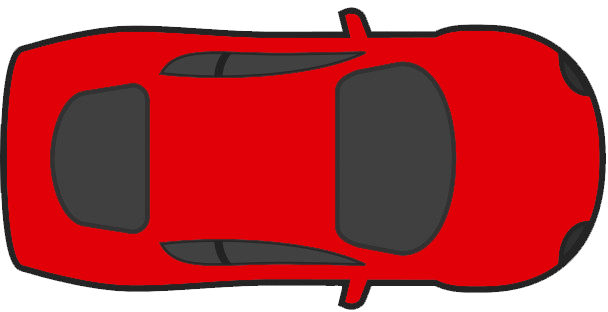
\includegraphics[width = 1.2cm]{img/car.png}};
}

\foreach \x in {5.2, 6.8, ..., 7.5}
{
	\node at (\x, 0.5) {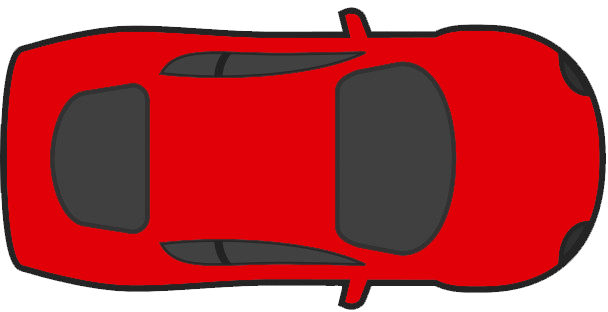
\includegraphics[width = 1.2cm]{img/car.png}};
}

\draw[blue, thick] (2.35, -0.2)
	node[below] {$+q(u(x+h), t)$}
	-- (2.35, 1.2) node[anchor = south west] {$x$};
\draw[blue, thick] (4.55, -0.2)
	node [below] {$- q(u(x + h,t))$}
	 -- (4.55, 1.2) node[anchor = south west] {$x+h$};
\end{tikzpicture}
